\documentclass{article}

% For adjusting images
\usepackage{adjustbox}
% For functions like \binom
\usepackage{amsmath}
% For functions like \wedge \subseteq \mathbb
\usepackage{amssymb}
% 312 Font
\usepackage{charter}
% Circuit diagrams
\usepackage{circuitikz}
% Custom lists
\usepackage{enumitem}
% Page margins & pagestyles
\usepackage{fullpage}
% Font encoding
\usepackage[T1]{fontenc}
% Hyperlinks
\usepackage{hyperref}
% Colored boxes around the 'solution' environment
\usepackage{mdframed}
% For color
\usepackage{xcolor}

% Defines a solution environment that creates a green box around text inside.
\mdfdefinestyle{SolutionFrame}{linecolor=green!60!black,linewidth=1pt}
\newenvironment{solution}{\begin{mdframed}[style=SolutionFrame]}{\end{mdframed}}

% Enumerate with (a),(b),(c),...
\newenvironment{enum}{\begin{enumerate}[label={(\alph*)}]}{\end{enumerate}}

% Set up hyperlinks
\hypersetup{
    colorlinks=true,
    urlcolor=white!30!blue
}

% Put a dot after section titles
\renewcommand\thesection{\arabic{section}.}
\renewcommand\thesubsection{\arabic{section}.\arabic{subsection}}
% Black footnotes
\renewcommand\thefootnote{\textcolor{black}{\arabic{footnote}}}
% Easier symbols
\newcommand\E{\mathbb{E}}
\renewcommand\P{\mathbb{P}}
\newcommand\N{\mathcal{N}}
\newcommand\Var{\text{Var}}
\newcommand\dx{\mathrm{d}x}
\newcommand\dy{\mathrm{d}y}

\newcommand\ds{\displaystyle}
\newcommand\bigger[1]{\ds#1\textstyle}

% Hide the Date
\date{}
% Hide page numbers
\pagenumbering{gobble}

\begin{document}
    \begin{titlepage}
        \centering
        \null
        \vspace{5cm}
        {\Huge CSE 369 Lab 1-2\par}
        \vspace{0.5cm}
        {\Large An Introduction to SystemVerilog and Digital Components \par}
        \vfill
        {\hfill \Large Isaac Wu \par}
        {\hfill \large 2360957 \par}
        {\hfill \large \today \par}
    \end{titlepage}

\section{SystemVerilog Design and Simulation}
    A simple, accurate explanation of what the mux4\_1 circuit does. Note: We do NOT want a written description of the circuit gates, we want a description of what it actually does – if you're not sure, see how we described how the mux2\_1 circuit works in Section 2 of the Quartus Tutorial.
    \begin{solution}
        mux4\_1 has 4 inputs: i00, i01, i10, i11, along with 2 select inputs: sel0 and sel1. Based on the selectors, the mux4\_1 circuit will match the corresponding input. sel0 represents the rightmost bit of the input and sel1 represents the left. For example, if sel0=0 and sel1=1, then mux4\_1=i10.
    \end{solution}

\section{Logic Investigation}
    \begin{enumerate}
        \item Which logical value (0 = FALSE = GND, 1 = TRUE = VDD) turns the red LEDs on?
            \begin{solution}
                1/VDD turns the red LEDs on.
            \end{solution}
        \item Which position (up or down) of the slider switch outputs a TRUE?
            \begin{solution}
                The up position of the slider outputs a TRUE.
            \end{solution}
        \item Which position of the push button (pressed or unpressed) outputs a TRUE?
            \begin{solution}
                The unpressed position of the push button outputs a TRUE.
            \end{solution}
    \end{enumerate}

\stepcounter{section}
\section{Digit Recognizer (Design)}
    1-digit recognizer circuit:
    \begin{solution}
        \begin{center}
            \begin{circuitikz} \draw
                (0,3) node (sw3) {SW3}
                (0,2) node (sw2) {SW2}
                (0,1) node (sw1) {SW1}
                (0,0) node (sw0) {SW0}
                (5,1.5) node (out) {LED}

                (1,3) node[not port, scale=0.75] (not) {}
                % (1,4) node[not port, scale=0.75] (not2) {}
                % (1,2) node[not port, scale=0.75] (not1) {}
                % (1,0) node[not port, scale=0.75] (not0) {}
                (3,2.5) node[nand port] (nand_32) {\hspace{-0.4em}\footnotesize NAND}
                (3,.5) node[nand port] (nand_10) {\hspace{-0.4em}\footnotesize NAND}
                (4.5,1.5) node[nor port] (nor) {\footnotesize NOR}

                (sw3) -- (not.in)
                (not.out) |- (nand_32.in 1)
                (sw2) -| (nand_32.in 2)
                (sw1) -| (nand_10.in 1)
                (sw0) -| (nand_10.in 2)
                (nand_32.out) -- (nor.in 1)
                (nand_10.out) -- (nor.in 2)
                (nor.out) -- (out);
            \end{circuitikz}
        \end{center}
    \end{solution}

% \newpage
\clearpage
\section{Multi-Digit Recognizer (Implementation)}
    A screenshot of the ModelSim simulation for your 2-digit recognizer design (always with explanation!).
    \begin{solution}
        Here is the code for my multi-digit recognizer. I defined two logic intermediaries to keep track if my input matches each digit. Then, I combined them and assigned them to the LED output.
        
        \begin{minipage}[t]{0.9\linewidth}
            \hspace{35pt}
            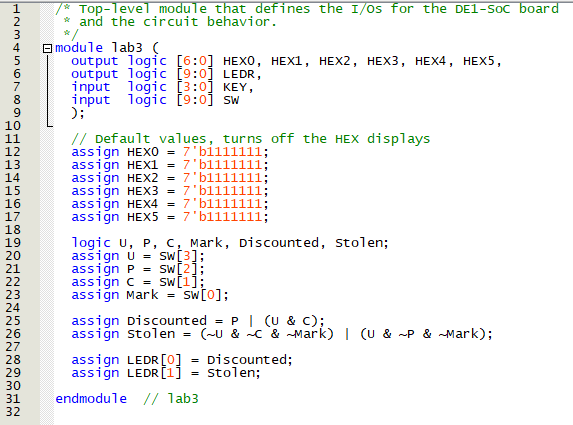
\includegraphics[width=0.9\linewidth]{code.png}
        \end{minipage}
        
        This is what my wave diagram looks like. The top 8 waves show the 8 switches alternating to test all 256 combinations. The bottom wave is the LED output, which is only true in one combination: 01010111.

        \begin{minipage}[t]{0.9\linewidth}
            \hspace{35pt}
            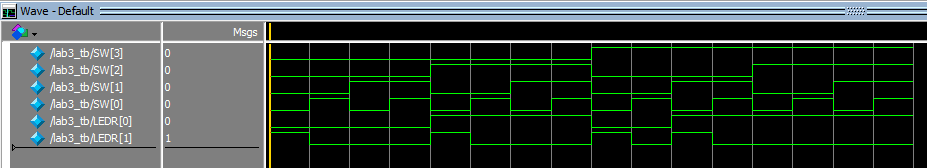
\includegraphics[width=0.9\linewidth]{waves.png}
        \end{minipage}
    \end{solution}

\section{Misc.}
    How many hours (estimated) it took to complete this lab in total, including reading, planning, designing, coding, debugging, and testing.
    \begin{solution}
        It took around 5-6 hours to complete this lab in its entirety.
    \end{solution}

\end{document}